\documentclass{beamer}
\usepackage[utf8]{inputenc}

\usetheme{Madrid}
\usecolortheme{default}
\usepackage{amsmath,amssymb,amsfonts,amsthm}
\usepackage{txfonts}
\usepackage{tkz-euclide}
\usepackage{listings}
\usepackage{adjustbox}
\usepackage{array}
\usepackage{tabularx}
\usepackage{gvv}
\usepackage{lmodern}
\usepackage{circuitikz}
\usepackage{tikz}
\usepackage{graphicx}
\usepackage{multicol}

\setbeamertemplate{page number in head/foot}[totalframenumber]

\usepackage{tcolorbox}
\tcbuselibrary{minted,breakable,xparse,skins}

\definecolor{bg}{gray}{0.95}
\DeclareTCBListing{mintedbox}{O{}m!O{}}{%
  breakable=true,
  listing engine=minted,
  listing only,
  minted language=#2,
  minted style=default,
  minted options={%
    linenos,
    gobble=0,
    breaklines=true,
    breakafter=,,
    fontsize=\small,
    numbersep=8pt,
    #1},
  boxsep=0pt,
  left skip=0pt,
  right skip=0pt,
  left=25pt,
  right=0pt,
  top=3pt,
  bottom=3pt,
  arc=5pt,
  leftrule=0pt,
  rightrule=0pt,
  bottomrule=2pt,
  toprule=2pt,
  colback=bg,
  colframe=orange!70,
  enhanced,
  overlay={%
    \begin{tcbclipinterior}
    \fill[orange!20!white] (frame.south west) rectangle ([xshift=20pt]frame.north west);
    \end{tcbclipinterior}},
  #3,
}
\lstset{
    language=C,
    basicstyle=\ttfamily\small,
    keywordstyle=\color{blue},
    stringstyle=\color{orange},
    commentstyle=\color{green!60!black},
    numbers=left,
    numberstyle=\tiny\color{gray},
    breaklines=true,
    showstringspaces=false,
}

\title 
{4.8.25}
\date{}

\author
{SAMYAK GONDANE - AI25BTECH11029}

\begin{document}

\frame{\titlepage}

\begin{frame}{Question}
Find the coordinates of the foot of the perpendicular drawn from the point $\vec{A}(-1, 8, 4)$ to the line joining the points $\vec{B}(0, -1, 3)$ and $\vec{C}(2, -3, -1)$. Hence find the image of the point $\vec{A}$ in the line $BC$.
\end{frame}

\begin{frame}{Solution}
\textbf{Direction Vector of Line BC}
\begin{align}
\vec{d} = \vec{C} - \vec{B} = 
\myvec{2 \\ -3 \\ -1} - \myvec{0 \\ -1 \\ 3} = \myvec{2 \\ -2 \\ -4}
\end{align}

\textbf{Parametric Form of Line BC}
\begin{align}
\vec{r}(t) = \vec{B} + t\vec{d} = 
\myvec{
0 \\ -1 \\ 3
}
+ t
\myvec{
2 \\ -2 \\ -4
}
=
\myvec{
2t \\ -1 - 2t \\ 3 - 4t
}
\end{align}
\end{frame}

\begin{frame}{Solution}
\textbf{Orthogonality Condition}
\begin{align}
\vec{r}(t) - \vec{A} =
\myvec{2t + 1 \\ -2t - 9 \\ -4t - 1}
\end{align}

$$(\vec{r}(t) - \vec{A}) \cdot \vec{d} = 0$$

\begin{align}
(2t + 1)(2) + (-2t - 9)(-2) + (-4t - 1)(-4) = 0 \\
4t + 2 + 4t + 18 + 16t + 4 = 0 \\
24t + 24 = 0 \Rightarrow t = -1
\end{align}
\end{frame}

\begin{frame}{Solution}
\textbf{Foot of Perpendicular}
\begin{align}
\vec{r}(-1) = 
\myvec{0 \\ -1 \\ 3}
+ (-1)
\myvec{2 \\ -2 \\ -4}
=
\myvec{-2 \\ 1 \\ 7}
\end{align}

\textbf{Image of A in Line BC}
\begin{align}
\vec{A}_{\text{image}} = 2\vec{r}_{\perp} - \vec{A} =
2
\myvec{-2 \\ 1 \\ 7}
-
\myvec{-1 \\ 8 \\ 4}\\
=
\myvec{-4 \\ 2 \\ 14}
+
\myvec{1 \\ -8 \\ -4}
=
\myvec{-3 \\ -6 \\ 10}
\end{align}
\end{frame}

\begin{frame}{Plot}
\begin{figure}[H]
    \centering
    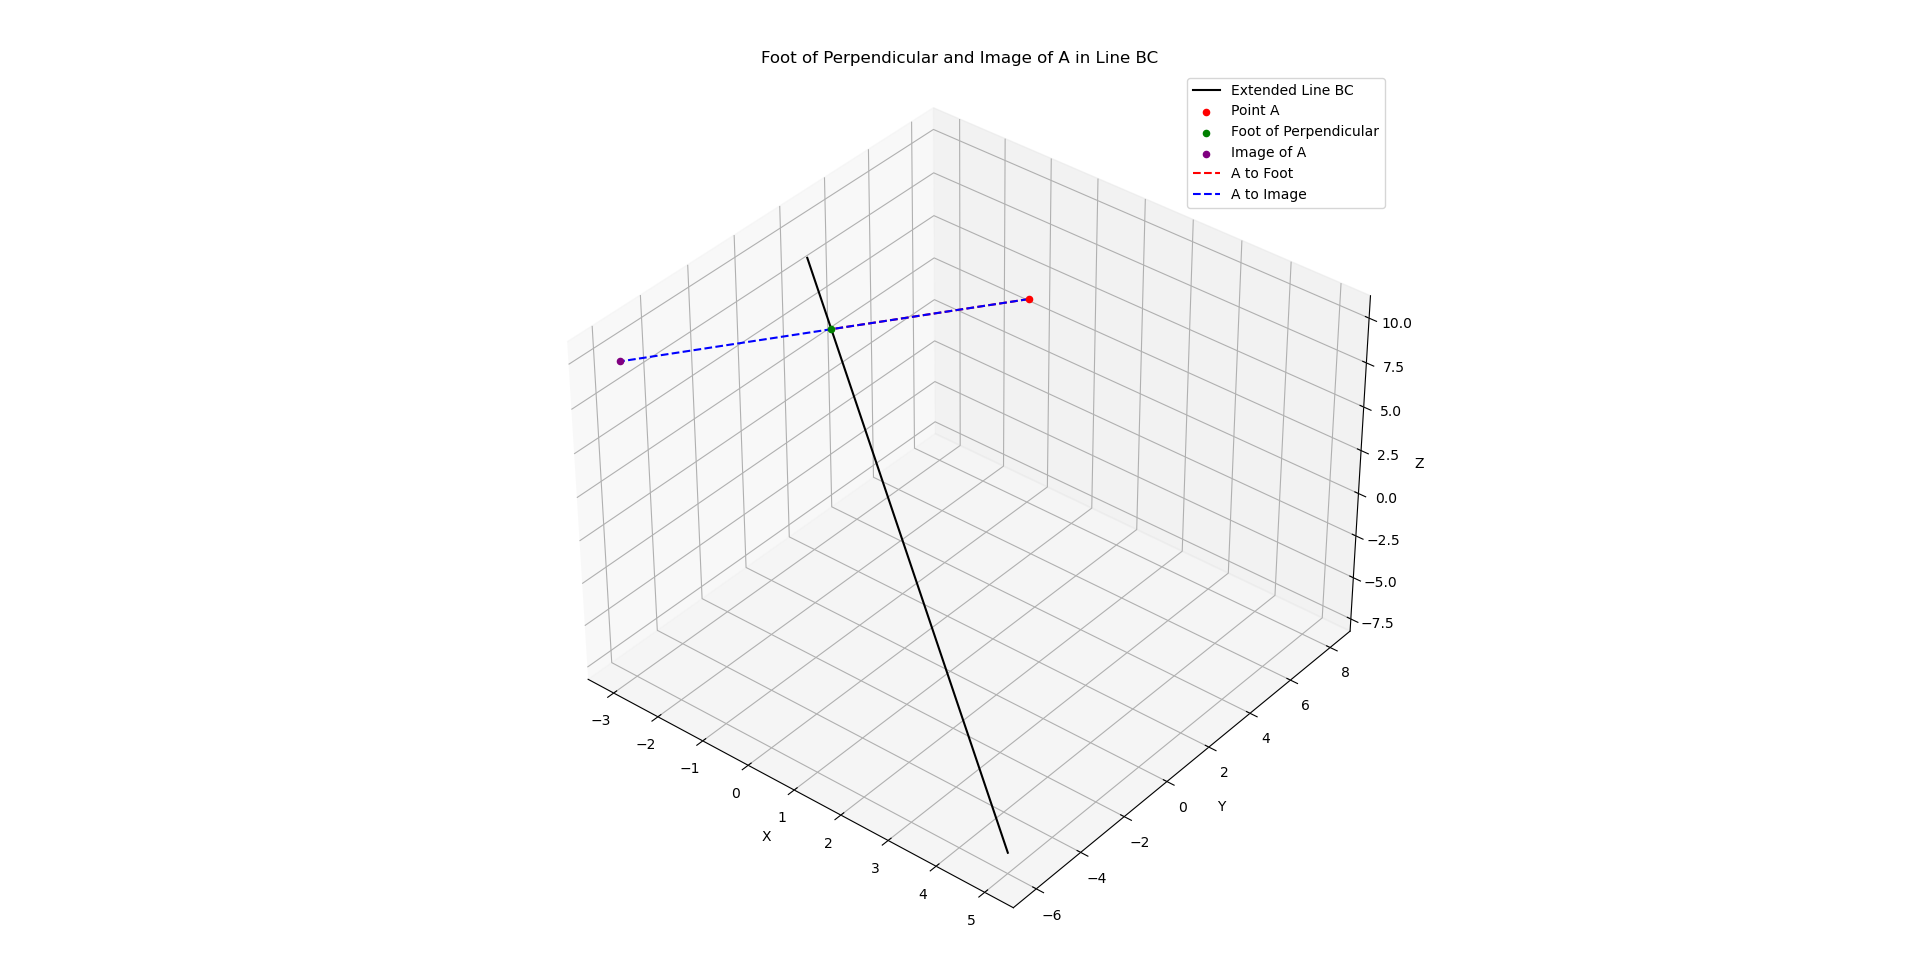
\includegraphics[width=1\linewidth]{./figs/Figure_1.png}
    \caption{}
    \label{fig:fig1}
\end{figure}
\end{frame}

\end{document}